\documentclass[11pt,a4paper]{article}
\usepackage[margin=2.5cm]{geometry}
\usepackage{booktabs,listings,xcolor,hyperref,tikz}
\usetikzlibrary{positioning,arrows.meta}
\lstset{basicstyle=\ttfamily\small,frame=single,breaklines=true,columns=fullflexible}
\hypersetup{colorlinks=true,urlcolor=blue}

\title{A RISC-V SoC with a Hardware Accelerator\\on the Tang Nano 9K}
\author{Parth Sinha}
\date{\today}

\begin{document}
\maketitle

\begin{abstract}
A small system-on-chip built entirely with open-source tools on a Sipeed Tang Nano 9K (Gowin GW1NR-9).
A PicoRV32 RISC-V core runs C firmware from 16\,KB of block RAM, talks to a PC over a hardware UART,
and offloads a pseudo-random-number generator to a memory-mapped accelerator.
On the real board the accelerator ran 1000 xorshift32 steps in 1066 cycles against 50015 in software, a $46\times$ reduction.
Source: \url{https://github.com/sinhaparth5/tangnano9k-riscv-soc}.
\end{abstract}

\section{Architecture}
\begin{center}
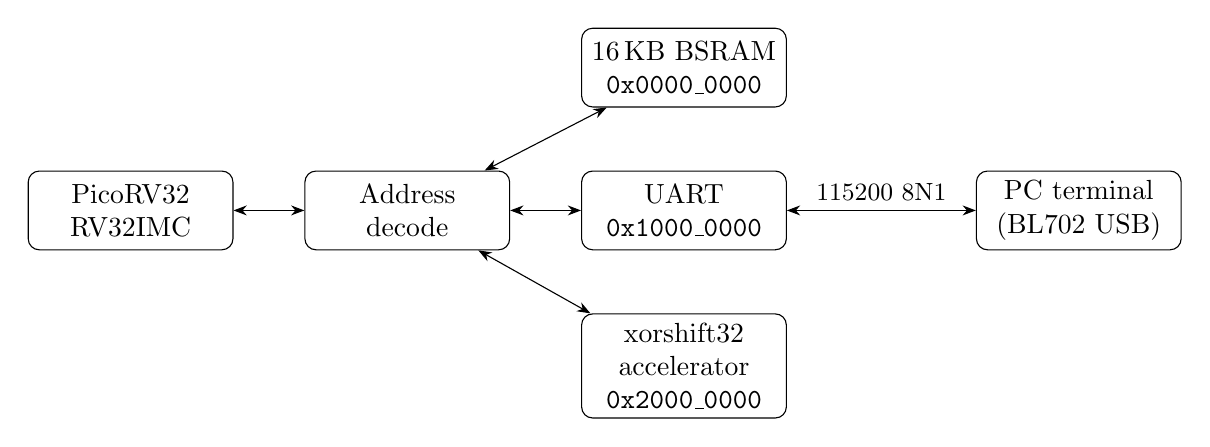
\begin{tikzpicture}[node distance=8mm and 9mm,
  blk/.style={draw,rounded corners,minimum width=2.6cm,minimum height=1.0cm,align=center},
  >={Stealth}]
  \node[blk] (cpu) {PicoRV32\\RV32IMC};
  \node[blk,right=of cpu] (dec) {Address\\decode};
  \node[blk,above right=of dec] (ram) {16\,KB BSRAM\\\texttt{0x0000\_0000}};
  \node[blk,right=of dec] (uart) {UART\\\texttt{0x1000\_0000}};
  \node[blk,below right=of dec] (acc) {xorshift32\\accelerator\\\texttt{0x2000\_0000}};
  \node[blk,right=24mm of uart] (pc) {PC terminal\\(BL702 USB)};
  \draw[<->] (cpu) -- (dec);
  \draw[<->] (dec) -- (ram);
  \draw[<->] (dec) -- (uart);
  \draw[<->] (dec) -- (acc);
  \draw[<->] (uart) -- node[above]{\small 115200 8N1} (pc);
\end{tikzpicture}
\end{center}
The CPU uses PicoRV32's native memory interface with one wait state on every access.
The 27\,MHz board oscillator is used directly, with no PLL.

\subsection{Memory map}
\begin{tabular}{@{}lll@{}}\toprule
Address & Register & Access\\\midrule
\texttt{0x0000\_0000}--\texttt{0x0000\_3FFF} & RAM (code, data, stack) & R/W\\
\texttt{0x1000\_0000} & UART data: write sends a byte, read pops the RX FIFO & R/W\\
\texttt{0x1000\_0004} & UART status: bit 0 TX busy, bit 1 RX not empty & R\\
\texttt{0x2000\_0000} & Accelerator \texttt{X}: PRNG state and result & R/W\\
\texttt{0x2000\_0004} & \texttt{N}: number of steps & W\\
\texttt{0x2000\_0008} & \texttt{CTRL}: bit 0 starts a run & W\\
\texttt{0x2000\_000C} & \texttt{STATUS}: bit 0 busy & R\\\bottomrule
\end{tabular}

\subsection{Accelerator}
The accelerator advances a 32-bit xorshift state ($x \mathrel{\oplus}= x\ll13$; $x \mathrel{\oplus}= x\gg17$; $x \mathrel{\oplus}= x\ll5$) once per clock for $N$ clocks.
The CPU writes \texttt{X} and \texttt{N}, sets \texttt{CTRL}, polls \texttt{STATUS}, then reads \texttt{X}.

\section{Toolchain}
Yosys (synthesis), nextpnr-himbaechel (place and route), Apicula \texttt{gowin\_pack} (bitstream), openFPGALoader (programming),
Icarus Verilog (simulation) and \texttt{riscv64-unknown-elf-gcc} with \texttt{-march=rv32imc -mabi=ilp32} for firmware.
One Makefile drives everything: \texttt{make PHASE=p4\_accel [sim|prog|flash]}.
Firmware is compiled, converted to a one-word-per-line hex file with \texttt{objcopy} and \texttt{od}, and loaded into the RAM at synthesis time with \texttt{\$readmemh}.

\section{Phases and verification}
\begin{tabular}{@{}llp{7.4cm}@{}}\toprule
Phase & Design & Verified\\\midrule
1 & LED counter & On board: six LEDs count in binary\\
2 & UART echo & Simulation loopback test; on board: typed characters echo\\
3 & PicoRV32, RAM, UART & Simulation runs the real firmware and checks the prompt; on board: banner and prompt appear\\
4 & Accelerator and shell & Simulation checks \texttt{seed}, \texttt{rand}, \texttt{peek}; on board: \texttt{rand}, \texttt{seed}, \texttt{bench}, \texttt{peek}\\\bottomrule
\end{tabular}

\medskip\noindent The Phase 4 shell offers \texttt{help}, \texttt{rand [n]}, \texttt{seed <hex>}, \texttt{bench [n]}, \texttt{peek <addr>}, \texttt{poke <addr> <val>} and \texttt{cycles}.
Results were checked against an independent Python implementation: five steps from seed 1 give \texttt{8ef917d1}, ten steps give \texttt{add02374}, and both matched on the board.

\section{Results}
\subsection{Resources}
nextpnr place-and-route reports for the GW1NR-9 (8640 LUT4, 6480 DFF, 26 BSRAM):
\begin{center}
\begin{tabular}{@{}lrrrr@{}}\toprule
Phase & LUT4 & DFF & BSRAM & $F_{\max}$ (MHz)\\\midrule
1 LED counter & 33 & -- & 0 & 239\\
2 UART echo & 119 & 50 & 0 & 141\\
3 CPU + UART & 4113 (47\%) & 1327 & 8 & 51\\
4 + accelerator & 4019 (46\%) & 1455 & 8 & 53\\\bottomrule
\end{tabular}
\end{center}
Phase 4 also uses 850 ALU blocks (13\%) and 40 RAM16SDP4 (14\%); no hardware multipliers are used.
The CPU uses more logic than the 2000--3500 LUT4 first estimated, because the multiplier, divider and compressed-instruction decoder are all enabled.
$F_{\max}$ is the post-route figure from nextpnr, which targeted its default 12\,MHz because no clock constraint is given; every design clears the real 27\,MHz clock by a wide margin.

\subsection{Accelerator benchmark}
Measured on the board with \texttt{bench 1000}, using the CPU \texttt{rdcycle} counter:
\begin{center}
\begin{tabular}{@{}lrr@{}}\toprule
 & Cycles & Per step\\\midrule
Software loop & 50015 & 50\\
Accelerator (including MMIO) & 1066 & 1.07\\
Reduction & \multicolumn{2}{c}{$46\times$, results identical}\\\bottomrule
\end{tabular}
\end{center}
The accelerator itself takes one cycle per step, so about 66 of the 1066 cycles are bus overhead (three register writes, a polling loop and a read).
This suggests a speedup of roughly $50N/(N+66)$ for $N$ steps, which would be below $1\times$ for single steps and approach $50\times$ for long runs. This is a model fitted to one measurement, not measured at other $N$.

\section{Problems met on the way}
\begin{itemize}
\item \textbf{Linux ModemManager corrupted the console.} After each load it probed the USB serial port and the board received its own banner and prompts as typed input, so a line such as \texttt{cycles} arrived as \texttt{> cycles} and was rejected. Fixed with a udev rule that sets \texttt{ID\_MM\_DEVICE\_IGNORE=1} for the FTDI device.
\item \textbf{Backspace bug.} A Backspace on an empty line was stored as a character. The simulation test now sends one Backspace first (two would cancel each other out and hide the bug).
\item \textbf{Failed flash verification.} One \texttt{flash} reported a CRC failure and the board then misbehaved after power-up; reflashing a known-good image succeeded. Loading to SRAM with \texttt{prog} is the safe default while developing.
\item \textbf{Serial port disappears on programming.} Each JTAG load re-enumerates the USB device, so a terminal opened before loading goes stale. Open the terminal after loading.
\item \textbf{Simulation versus board.} The testbench initially passed with a broken design because of a race on the start signal and a string truncated by an undersized vector; both were test bugs found by checking that the test fails on bad input.
\end{itemize}

\section{Limitations and next steps}
The UART receive FIFO holds 64 bytes and drops the newest byte on overflow. \texttt{poke} and \texttt{peek} do no address checking, so a write into RAM can crash the program.
Possible extensions: a MicroSD SPI controller, an HDMI/DVI frame buffer, or a small scheduler on the CPU. None of these is started.

\end{document}
